\section{Creating the Decision Support System}
\subsection{Choosing a problem}
The first step in solving the task for creating a decision support system is
selecting a problem for the system to solve. I have chosen to let the system
help in deciding the every-day-decision of what to do now, for a
regular student. For this kind of system, it is really hard to get real values
for the utility function, and also difficult to set default probabilities for
the environment. These values and probabilites must also be adjusted for each
subject, as different persons have different personalities, preferences and
work-effectiveness.


I have chosen the following activities that the system will help you decide
between:
\begin{itemize}
  \item Watch a movie with someone
  \item Watch a movie alone
  \item Do homework
  \item Eat dinner with someone
  \item Eat dinner alone
  \item Go to sleep
  \item Go outside
  \item Do excercise
\end{itemize}
of coure, there are a lot more things that could be added, but I think these are
a representative overall of actions.

\subsection{Decision parameters}
\index{parameters}Now that we have our problem defined, we need information
about the current state, in order to promote a good decision.

I have chosen some attributes that I think is important in order to decide what
to do, in the general context.

\begin{description}
\item[Lot to do] \hfill \\
Students have a \index{lot to do}lot to do, occasionally, but may also have a
lot of spare time.
Because how much you have to do is important deciding if you should do homework,
I have included this parameter.

\item[Hungry] \hfill \\
Whenever you are \index{hungry}hungry, it is a good idea to eat food.

\item[Sleepy] \hfill \\
You might be better off with sleeping than doing homework or doing excercises if
you are \index{sleepy}sleepy.

\item[Tired] \hfill \\
\index{tired}Tired is kind of a extended expression for sleepy, hungry, but also
general ``don't want to do nothing''. I have included this as a way of telling you are
tired, without beeing explicitly sleepy. If you are sleepy, of cource, this
affects tired, unless specified otherwise.

\item[Social needs] \hfill \\
Everyone has social needs from time to time, but sometimes, we also prefer
beeing alone. This is important deciding wherever we are going to spend time
alone, or meeting other people.

\item[Weather] \hfill \\
The \index{weather}weather is more an environmental condition, but is also
important for some decisions. We might say that it is more pleasing going out on a sunny
afternoon, then if it is a full storm outside. I would also state that there are
somewhat better to do homework while it is raining outside, since it lowers the
desire to go outside.

\end{description}

\subsection{The effect of a choise}
In order to calculate the \index{utility}utility value of a choise, we have to
look at its consequences. I have chosen some attributes that work as outcome of a choise and
a state. I have chosen to include the following consequence variables:
\begin{description}
\item[Usefullness] \hfill\\
I will argue that you feel better if you have done something usefull. Something
usefull depends on what demands you were having before doing an action, eg. if
you where hungry, it may be more usefull to eat something than to watch a movie,
and if you had a lot to do, it might be most usefull to do some homework.

\item[Work left] \hfill\\
How much work are we left with after doing our action. This is important because
it may be difficult to relax if you have much on your mind. Typically doing
homework leaves you with less to do, while sleeping leaves you with exactly the
same amout.

\item[Exhausting] \hfill\\
You might be more pleased with yourself if you have done something that was not
exhausting, since it leaves you with more energy. You might argue that it feels
good to be real exhausted after a hard excercise, but I have put those values
into \emph{Usefullness}, leaving just ``bad'' exhaustnes into this variable.

\item[Fun] \hfill\\
The more fun we have had, the better. Often, fun goes against usefullness, but
since some things might be fun and usefull, we need both variables.

\item[Social] \hfill\\
People have social demands, and this is important to how good we feel. If we
have little contact with other human beeings, we might feel lonely, while
over-stimulating the social life might not be too good either.

\item[Hunger] \hfill\\
Even though we allready have the state node Hungry, we need to know how hungry
we will be given a decision. Since mood is much dependent on hunger, this is an
important node.

\item[Physiological feeling] \hfill\\
This node is a merge between Exhausting, Fun, Social and Hunger, since I think
all these represents how good your body feels. Fun and Social might be argued,
but if you feel that you have a lot of friends, or you feel that this is a lot
of fun, you tend to forget about hunger and exhastness. Because of that, we may
combine these into one node, both simplifing the model and the caluculations.

\end{description}

\subsection{Compiling variables into a system}
The previous sections defined a set of variables and a set of choises that
makes up to a \index{mini-world}mini-world. The consepts of mini-worlds is that
they models the real world, or any world where we want to do computations. Of course, a more
advanced mini-world would be able to model the real world with better accuracy,
but would also (potensially) add severe complexity.

But since we have defined what our model contains, we have to model the
releations between the different attibutes. I want to do this in a way such that
the attributes and their relations make up a \index{Bayesian
network}\emph{Bayesian network}, since this is a datastructure that eases the
computation needs in opposition to a \index{truth table} \emph{truth
table}\cite{aima}. The consept of easing the computational needs in the Bayesian
network is called \emph{conditional independence}\index{conditional
independence}. What it means, is basicaly that a node is self-contained given
its parents, and we do not need to go further on to grand parents and so on to
find its real value. This is an assumption that we must take to avoid large
tables, and is a property of the Bayesian Network.

An example of a \emph{Bayesian network} is included in
Figure~\ref{fig:BayExample}.
\begin{figure}[h]
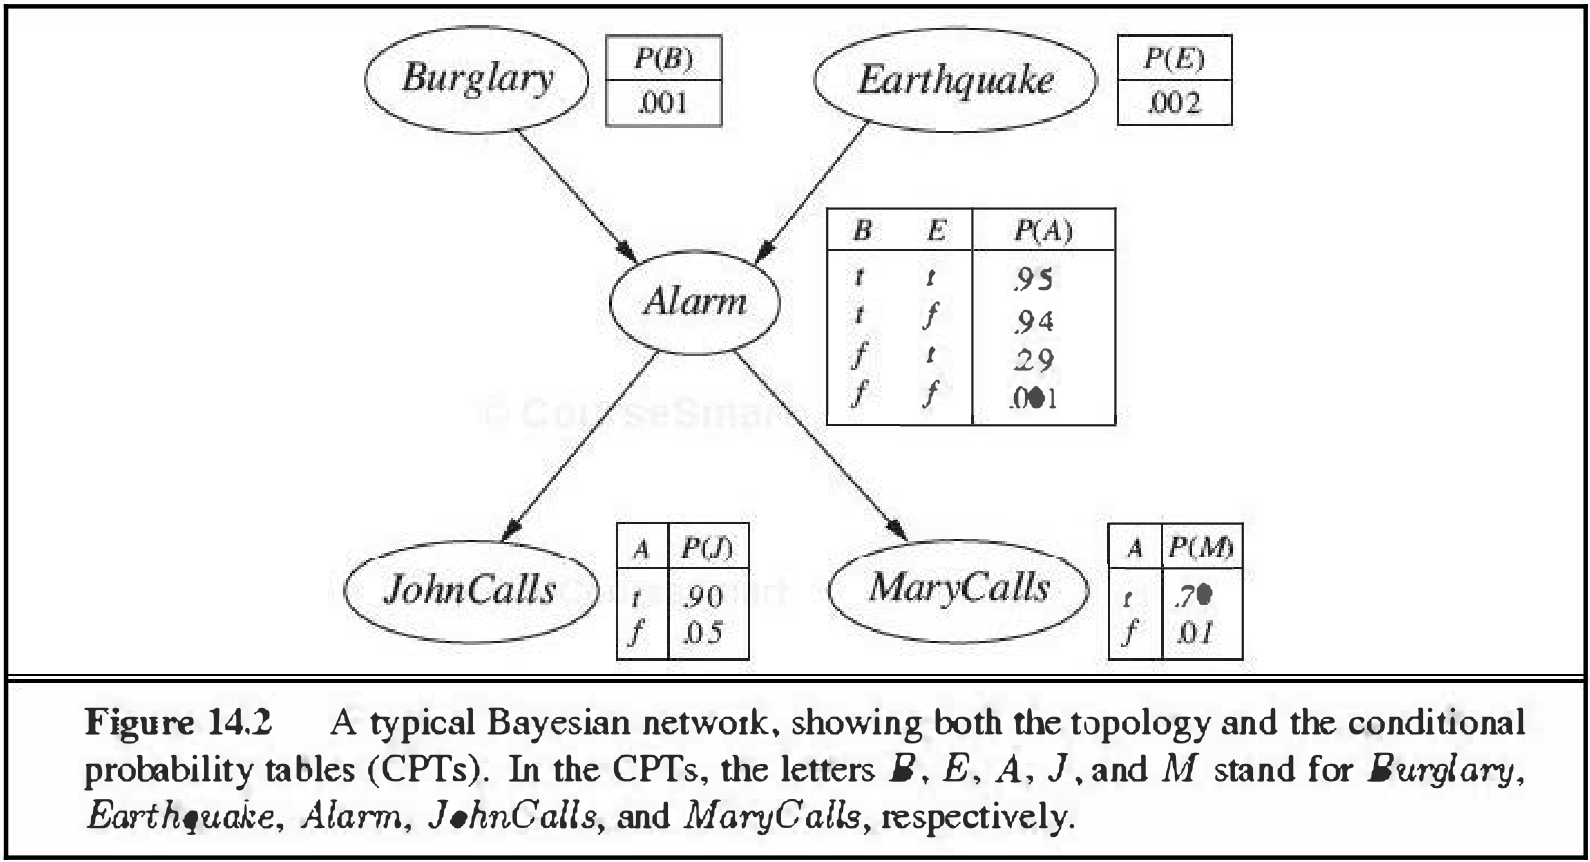
\includegraphics[width=122mm]{figure-example1.png}
\caption{Example of Bayesian network, copy of figure from AIMA\cite{aima}}
\label{fig:BayExample}
\end{figure}
We see that the nodes represents states and actions, each with probabilities
that links together to a system.

From this, we can set up a system that maximizes the \emph{utility
value}\cite{aima} in such a way that it will chose those options with best
outcome. Again, the AIMA-book has a great example of such a system, and I have
included this in Figure~\ref{fig:dssExample}.
\begin{figure}[h]
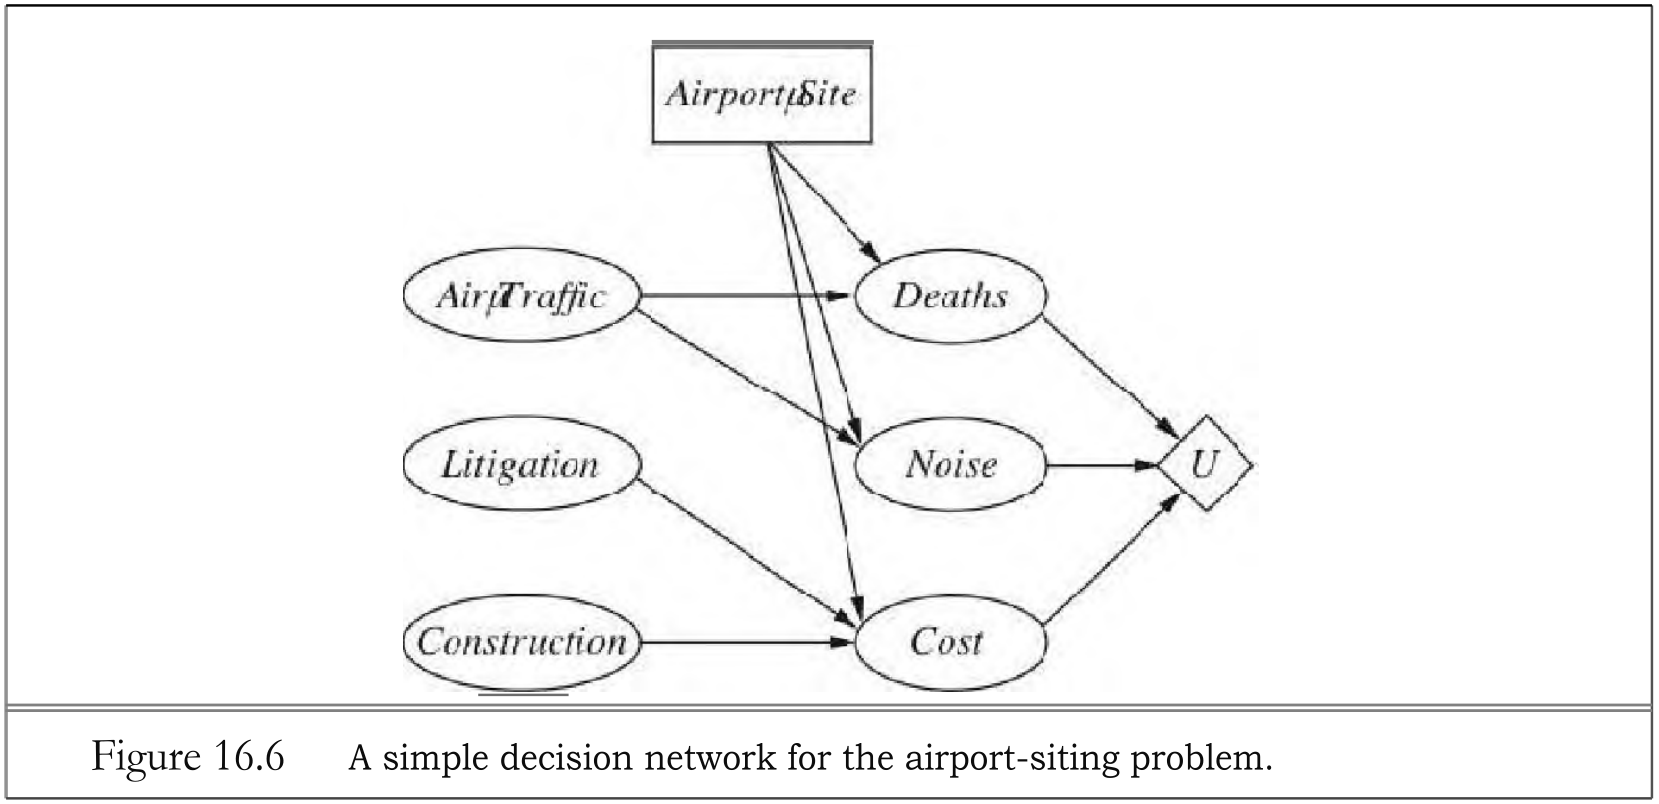
\includegraphics[width=122mm]{figure-example2.png}
\caption{Example of a desicion support system, copy of figure from
AIMA\cite{aima}}
\label{fig:dssExample}
\end{figure}

Now, our job will be to link the nodes that represents state and consequences
into a network like that. A screenshot from my complete model from GeNIe 2.0
is included as Figure~\ref{fig:complete}

Most of the work with setting up such a system, at least if you have a software
like GeNIe\footnote{\url{http://genie.sis.pitt.edu/}}, is filling the
\emph{truth tables}. I mentioned that Bayesian networks are better than large
truth tables, but they does not eliminate them. A \index{Bayesian
network}Bayesian network helps us minimizing the tables so that only related
properties gets computed together. In the real world, we might have a tight or
loose coupling between almost anything, in our mini-world, we separate the
attributes from each other, again to simplify computation.


The nodes marked as gray in Figure~\ref{fig:complete} is the state nodes. These
have simple tables, like this:
\begin{table}[h!!!!!!!!!!]
\begin{tabular}{|c|c|}
\hline
\multicolumn{2}{|c|}{Hungry}\\
\hline
Yes & 0.2\\
Some & 0.3\\
No & 0.5\\
\hline
\end{tabular}
\caption{Values from Hungry-node}
\label{tab:hungry}
\end{table}

The nodes marked as green are the state-nodes, which are affected by both
the state nodes and the decision\footnote{The large square node, coloured
light blue, stating ``What should I do now?''}. These nodes expand exponentially for
each parent connection, and will occationally grow large. The good thing with
the \emph{Bayesian network} is that we reduce the tables extremely much from
what they could have been if all values where to be stored in one table.

One of my tables with multiple parents looks like this:
\begin{table}[h!!!!!!!!!!!!!!!!!!]
\begin{tabular}{|c|c||c|c|c|}
\hline
\multicolumn{2}{|c|}{} & \multicolumn{3}{|c|}{Exhausting}\\
\hline
What to do & Tired & Yes & Some & No \\
\hline
\hline
Watch movie together & No & 0 & 0.1 & 0.9\\
Watch movie together & Some & 0.1 & 0.2 & 0.7\\
Watch movie together & Yes & 0.2 & 0.4 & 0.4\\
\hline
Watch movie alone & No & 0 & 0 & 1\\
Watch movie alone & Some & 0 & 0.1 & 0.9\\
Watch movie alone & Yes & 0.1 & 0.1 & 0.8\\
\hline
\multicolumn{5}{c}{\ldots}\\
\end{tabular}
\caption{Some values from the Exhausting-node}
\label{tab:exhaust}
\end{table}

with appropriate values for all decisions combined with the value of the state
nodes. All values are defined in the the GeNIe network attached with this
document.

\subsection{The utility}
This system calculates a value that we call the systems Utility Value. This
value tells us how appropriate the given situation is. If we have already
observed some variables or made a decision, the utility function takes this as
input and will tell us how good the current given situation is. The utility
function uses numbers from a table simmilar to the table above to weight the
outcome. The values from my utility function can be found in Table
\ref{tab:utility}. All the values are my opinion on a given decision combined
with the set of consequences. A value of 1 is perfect, while a value of 0 means
a situation I want to avoid. The numbers of the utility function are not limted
to the range between 0 and 1, like the chance nodes, because it works more like
a score. I like the range between 0 and 1 because it set limits for best and
worst, and I think that makes it easier to express the values of situations.

\subsection{Finding the right values}
But what are all these values? These values are the probability of a
state, or the probability of a consequense, given a descision and a state. Eg.
how likely is it that we become exhausted given that we watch a movie together
and we are tired already? This is the number in first column and third row in
the table above. Each row make up probabilities for given situations, and since
all possible situations are included, they must add up to one.

Allmost all the values in my decision support system are made up of my own
opinions of things. An exception is the weather node, where I have calculated
values from weather statistics\cite{met}. Those values are stated in Table
\ref{tab:weather}.
\begin{table}[h!!!]
\begin{tabular}{|c|c|}
\hline
\multicolumn{2}{|c|}{Weather}\\
\hline
Sunny & 0.4605757196\\
Cloudy & 0.2152690864\\
Rainy & 0.1739674593\\
Snowing & 0.1326658323\\
Storm & 0.0175219024\\
\hline
\end{tabular}
\caption{The Weather node, values calculated from met.no\cite{met}}
\label{tab:weather}
\end{table}
More state-node examples can be found in Table~\ref{tab:hungry} and Table
\ref{tab:sleepy} Examples of other values, that are entirely my opinion on state
and consequences can be found in Table~\ref{tab:exhaust}, but these tables are
so large that I have chosen not to include too much of them. Entire tables with
values can be found in the GeNIe-file attached with this document.
\begin{table}
\begin{tabular}{|c|c|}
\hline
\multicolumn{2}{|c|}{Sleepy}\\
\hline
Yes & 0.2\\
some & 0.2\\
No & 0.6\\
\hline
\end{tabular}
\caption{Values from the Sleepy-node}
\label{tab:sleepy}
\end{table}

\subsection{Connection of the nodes}
Now I will describe how I connected the nodes, and explain some of my choises.
As we see from Figure~\ref{fig:complete}, I have devided the world into state
(observed), decision and consequences(unobserved) parts. The chosen colours are
for just to tell the realms apart. I think that your mood depends highly on
those variables, and your best choise is highly dependent on your mood. The
values, again, are mostly chosen by how I see the world, and must be adjusted
for other personalities. By example, having an infant at home usually makes the
night shorter, and makes me more sleepy and tired than the average person. That
is why my Sleepy-values are higher than it would be if you just were sleepy a
few hours before bed-time. I also have connected Usefullness with Hungry, Sleepy
and Lot to do, because if you are hungry, it may be more usefull to eat than to
do anything else, same for sleepy and go to sleep. I you have nothing else to
do, anything may be usefull, but having a lot to do, in other words, home work,
then that must be done before watching a movie.

Likewise, how much work you have left leans on how much you have to do, how
tired you are, and what you choose to do. Sleeping or watching movies leaves you
with the same amount, while doing homework leaves you with somewhat less,
depending on how tired you were before starting.

How much fun you have depends highly on what you do alone, but also depends on
various factors. I have chosen to set your social needs and the weather as main
parameters, since going outside might be bad if there is a full storm outside,
and watching a movie with someone may also be bad if you just want to be alone.

Your social requirements are a major part of how good you feel, so if there was
any unmet social needs, that will count bad for the utility function. The social
requirements lean mostly on what you do, and how social you felt before doing
something.

I have chosen to link the four nodes Hunger, Exhausted, Fun and Social into
Physio logical feeling because I think they represent the way your body feels.
Linking them into one node makes the utility node's value table a lot
smaller\footnote{From 243 to 27 different values}, without lowering the acurracy
that much. This is one example of \index{conditional independence}conditional
independence, where you know how your body feels given Hunger, Exhausted, Fun
and Social, and there is no need for knowing what choises has been maid,
neither what state we had before making a decision.

\begin{figure}[h]
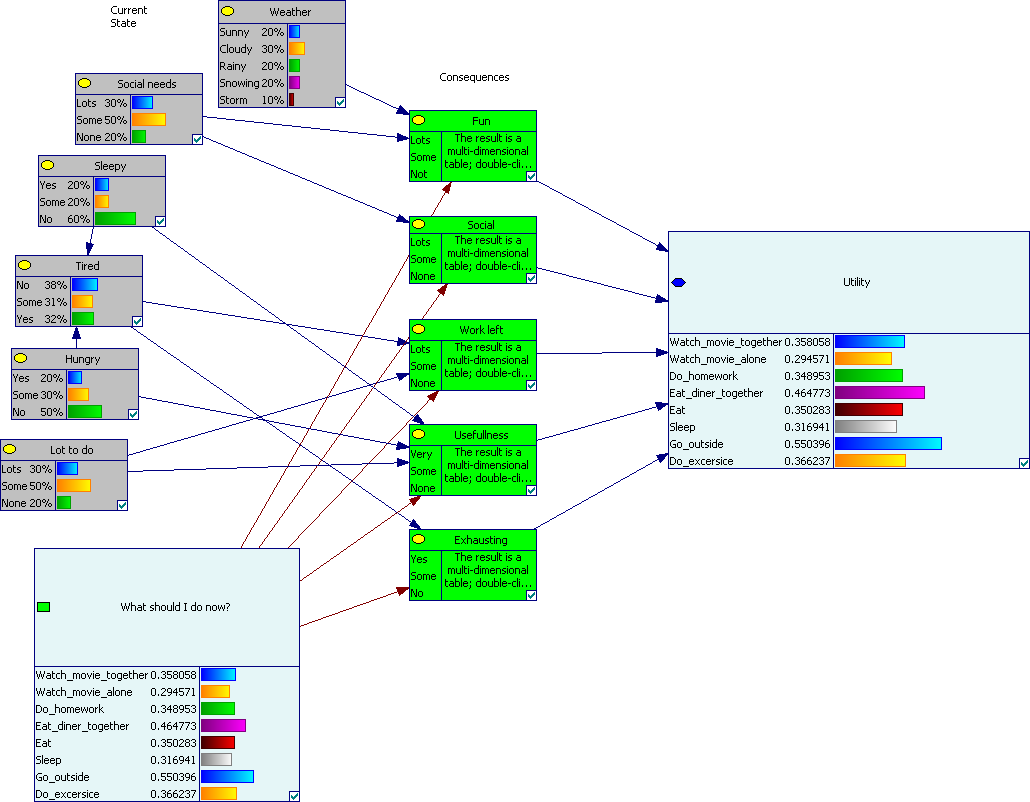
\includegraphics[width=154mm]{figure-complete.png}
\caption{Complete Decision Support System in GeNIe 2.0}
\label{fig:complete}
\end{figure}

\subsection{Observations and adjustments}
After filling in all probability tables and values of the utility function, we
still have a lot to do. These kind of systems needs to be adjusted so that they
agree with the target. In real systems, it is usual to compare the decision of
the sstem with a ``golden state'', that is the decision made from a group of
experts. In my system, I had to adjust the opinion-values until I felt I agreed
with the system. I learned that I usually had the utility value to high, and had
to lower many of them.

Some results from my system:\\
\begin{description}
\item[Hungry: No, Lot to do: Lots, Tired: No, Sleepy: no, Weather: Sunny,
Social needs: None]\\
Do homework has the highest utility, while go outside follows tight. This is
mostly because it is sunny outside.
\item[Hungry: No, Lot to do: Lots, Tired: No, Sleepy: no, Weather: Storm,
Social needs: None]\\
Setting weather to storm lowers the utility of go outside, while homework is
raised a little. This is because it is better to do homework when you don't want
to go outside anyways.
\item[Hungry: No, Lot to do: Lots, Tired: Yes, Sleepy: Yes, Weather: Sunny,
Social needs: None]\\
When you are sleepy and tired, it is better to go to sleep, rather than to do
homework. The utility of go outside is actually higher than do homework, this is
because you don't want to do homework when you are tired, since you don't learn
any thing, and things may be wrong, lowering your grade. Going out may give you
some energy, and it does not matter if you are tired. Anyways, sleep had a
governing utility here.
\end{description}


\begin{table}
\begin{tabular}{|c|c|c|c|c|c|}
\hline
Work left	&	Exhausting	&	Fun	&	Social	&	Usefulness	&	Value	\\
\hline
Lots	&	Yes	&	Lots	&	Lots	&	Very	&	0.4	\\
Lots	&	Yes	&	Lots	&	Lots	&	Some	&	0.2	\\
Lots	&	Yes	&	Lots	&	Lots	&	None	&	0.1	\\
Lots	&	Yes	&	Lots	&	Some	&	Very	&	0.5	\\
Lots	&	Yes	&	Lots	&	Some	&	Some	&	0.3	\\
Lots	&	Yes	&	Lots	&	Some	&	None	&	0.1	\\
Lots	&	Yes	&	Lots	&	None	&	Very	&	0.8	\\
Lots	&	Yes	&	Lots	&	None	&	Some	&	0.5	\\
Lots	&	Yes	&	Lots	&	None	&	None	&	0.3	\\
Lots	&	Yes	&	Some	&	Lots	&	Very	&	0.1	\\
Lots	&	Yes	&	Some	&	Lots	&	Some	&	0.1	\\
Lots	&	Yes	&	Some	&	Lots	&	None	&	0	\\
Lots	&	Yes	&	Some	&	Some	&	Very	&	0.2	\\
Lots	&	Yes	&	Some	&	Some	&	Some	&	0.2	\\
Lots	&	Yes	&	Some	&	Some	&	None	&	0	\\
Lots	&	Yes	&	Some	&	None	&	Very	&	0.3	\\
Lots	&	Yes	&	Some	&	None	&	Some	&	0.3	\\
Lots	&	Yes	&	Some	&	None	&	None	&	0	\\
Lots	&	Yes	&	Not	&	Lots	&	Very	&	1	\\
Lots	&	Yes	&	Not	&	Lots	&	Some	&	0	\\
Lots	&	Yes	&	Not	&	Lots	&	None	&	0	\\
Lots	&	Yes	&	Not	&	Some	&	Very	&	0.2	\\
Lots	&	Yes	&	Not	&	Some	&	Some	&	0.1	\\
Lots	&	Yes	&	Not	&	Some	&	None	&	0	\\
Lots	&	Yes	&	Not	&	None	&	Very	&	0.3	\\
Lots	&	Yes	&	Not	&	None	&	Some	&	0.2	\\
Lots	&	Yes	&	Not	&	None	&	None	&	0.1	\\
Lots	&	Some	&	Lots	&	Lots	&	Very	&	0.4	\\
Lots	&	Some	&	Lots	&	Lots	&	Some	&	0.3	\\
Lots	&	Some	&	Lots	&	Lots	&	None	&	0.1	\\
Lots	&	Some	&	Lots	&	Some	&	Very	&	0.5	\\
\ldots &\ldots &\ldots &\ldots &\ldots &\ldots \\
None	&	No	&	Some	&	Some	&	Some	&	0.6	\\
None	&	No	&	Some	&	Some	&	None	&	0.3	\\
None	&	No	&	Some	&	None	&	Very	&	0.8	\\
None	&	No	&	Some	&	None	&	Some	&	0.7	\\
None	&	No	&	Some	&	None	&	None	&	0.3	\\
None	&	No	&	Not	&	Lots	&	Very	&	0.3	\\
None	&	No	&	Not	&	Lots	&	Some	&	0.3	\\
None	&	No	&	Not	&	Lots	&	None	&	0.2	\\
None	&	No	&	Not	&	Some	&	Very	&	0.6	\\
None	&	No	&	Not	&	Some	&	Some	&	0.5	\\
None	&	No	&	Not	&	Some	&	None	&	0.4	\\
None	&	No	&	Not	&	None	&	Very	&	0.7	\\
None	&	No	&	Not	&	None	&	Some	&	0.6	\\
None	&	No	&	Not	&	None	&	None	&	0.5	\\
\hline
\end{tabular}
\label{Some values from the utility function}
\caption{Values of the utility function}
\label{tab:utility}
\end{table}
